% Potentially useful sources:
%   https://physics.stackexchange.com/questions/707380/is-lepton-flavour-universality-an-accidental-symmetry-of-the-standatd-model
%   https://physics.stackexchange.com/questions/672626/what-is-an-accidental-symmetry
%   https://physics.stackexchange.com/questions/55350/two-ways-to-form-su2-singlets
%   https://physics.stackexchange.com/questions/607444/chiral-symmetry
%   https://physics.stackexchange.com/questions/429180/how-does-bhabha-scattering-imply-the-existence-of-quark-lepton-substructure
%   https://physics.stackexchange.com/questions/96362/what-does-a-rm-su2-isospin doublet-really-mean
%   https://physics.stackexchange.com/questions/385159/quark-gluon-color-relationship-in-pure-qcd
%   https://physics.stackexchange.com/questions/327008/how-do-the-infinite-dimensional-representations-of-the-poincar%C3%A9-group-work
%   Rep. of Lorentz group: http://sharif.edu/~sadooghi/QFT-I-96-97-2/LorentzPoincareMaciejko.pdf
%
% Very useful:
%   https://physics.stackexchange.com/questions/266963/what-are-the-differences-if-any-between-the-dysons-series-definition-and-the
%   https://pages.cs.wisc.edu/~guild/symmetrycompsproject.pdf
%   https://physics.stackexchange.com/questions/578059/why-the-little-group-of-a-massless-spin 1-particle-is-iso2-rather-than-so2
%   https://math.stackexchange.com/questions/1334965/direct-sum-vs-direct-product-vs-tensor-product
%   https://physics.stackexchange.com/questions/619178/standard-model-notation-on-doublets
%   https://physics.stackexchange.com/questions/190416/what-role-does-spontaneous-symmetry-breaking-play-in-the-higgs-mechanism
%   https://physics.stackexchange.com/questions/316094/helicity-of-antiparticles
%
%   From Jack(!): https://physics.stackexchange.com/questions/92157/off-shell-corrections-to-massive-vector-boson-propagator-in-polarization-form
%
% Useful papers not cited:
%   On gauge symmetry: https://arxiv.org/pdf/1901.10420.pdf
%   2-component spinor notation: https://arxiv.org/pdf/0812.1594.pdf
%   V-A current: https://warwick.ac.uk/fac/sci/physics/staff/academic/boyd/stuff/neutrinolectures/weak.pdf
%   Review on V-A theory and chirality: https://www.hep.phy.cam.ac.uk/~thomson/lectures/partIIIparticles/Handout9_2009.pdf
%   Weak current: https://www.sciencedirect.com/science/article/pii/0550321389903064
%   Helicity amplitude: http://www-library.desy.de/preparch/desy/proc/proc13-03/Koerner.pdf


\chapter{Theory of semileptonic $B$ decays}
\label{ref:theory}

\section{Construction of the electroweak theory in the SM}

Through a close collaboration between experimentalists and theorists,
particle physicists were able to come up with a \emph{quantum field theory}
to describe \emph{interactions} of \emph{elementary particles},
known as the standard model of particle physics (SM).
A construction of the SM is outlined\footnote{
    ``I am an experimentalist!'' says the author waving his hands.
} first with the help of
\cite{Robinson_2011,Schwichtenberg_2018},
followed by brief discussions on quantum eletrodynamics (QED),
the electroweak theory, and the lepton flavor universality in the SM.


\subsection{Outline of the construction}

It is experimentally established that the speed of light in vacuum is constant
in any reference frame.
Then, all transformations preserving the speed of light\footnote{
    Each of such transformations, denote as $A$, must leave the Minkowski metric
    $\eta$ intact: $A^T \eta A = \eta$.
} can be identified:
rotations, Lorentz boosts, parity ($\vec{x} \rightarrow -\vec{x}$),
time reversal ($t \rightarrow -t$), and translations.
All but the translation transformations form a group called
``Lorentz group''.
Focusing on the restricted Lorentz group $SO^+(1, 3)$,
which preserves direction of space and time\footnote{
    Loosely speaking, Lorentz group contains 4 ``classes'': $\{I, T, P, TP\}$.
    $SO^+(1,3)$ is the one that contains the identity element.
    The other 3 can be obtained by applying parity ($P$), time reversal ($T$),
    or both ($TP$) to $SO^+(1,3)$.
},
and accepting that it is advantageous to extend $SO^+(1,3)$ to work with vectors
with complex components,
it is shown that the extended group, $SO^+(1,3)_\mathbb{C}$,
contains two copies of $SU(2)_\mathbb{C}$.
% SO+(1,3) = SU(2) x SU(2), direct product

One may ask the following question, then:
``What kinds of object does the group $SO^+(1,3)_\mathbb{C}$ act on?''
To answer this question, the group elements can be represented\footnote{
    With the understanding that any group element $\Lambda$ can be generated
    from 3 rotation generators $\vec{J}$ and 3 boost generators $\vec{K}$
    with the exponential map:
    $\Lambda = e^{i \vec{\theta} \cdot \vec{J} + i \vec{\phi} \cdot \vec{K}}$,
    and the commutation relations between the generators,
    namely $[J_i, J_j], [K_i, K_j], [J_i, K_j]$,
    can be worked out in any representation.
} by $n \times n$ matrices,
and the objects the group acts on by vectors of $n$ complex numbers.
Then the properties of a particular ``representation'' can be studied with
the familiar tool of linear algebra.
As a side note,
$SU(2)_\mathbb{C}$ can be represented by $2j + 1$ dimensional matrices,
where $j$ is a half-integer;
the $j = \frac{1}{2}$ case has 3 Pauli matrices as the group generators.
Since $SO^+(1,3)_\mathbb{C}$ contains two copies of $SU(2)_\mathbb{C}$,
its representations can be labelled as $(j, j')$.
It turns out the answer to the question at the beginning of the paragraph is:
each \emph{irreducible representation}\footnote{
    Roughly speaking, there is no transformation that can simultaneously
    block-diagonalize all matrices representing the group elements.
}
corresponds to a specific type of \emph{elementary particle}.
The $(0, 0)$ representation corresponds to spin 0 scalar particles;
the $(\frac{1}{2}, 0)$ and $(0, \frac{1}{2})$ representations both corresponds to
spin $\frac{1}{2}$ particles,
with the former left-handed and the latter right-handed;
the $(\frac{1}{2}, \frac{1}{2})$
representation corresponds to spin 1 particles.
There are many more irreducible representations,
but in the SM only the spin 0, $\frac{1}{2}$, and 1 particles are present.

Now the SM can be constructed as follows:
First, consider elementary particles with spin 0, $\frac{1}{2}$, and 1,
which are represented by linear operators in a space.
A Lorentz-invariant Lagrangian density\footnote{
    Will be referred to as ``Lagrangian'' in later text for brevity.
} can be built from
linear, quadratic, and the lowest possible derivative terms of these
operators.
A Lagrangian built in this manner contains no interaction (i.e. a free
Lagrangian).
Then, require the Lagrangian to be invariant\footnote{
    Speaking with a limited knowledge: local gauge invariances represent
    mathematical redundancy in the description of the system,
    and must be preserved to have a consistent theory.
} under certain local gauge transformations
such as that from $U(1), SU(2)$, and $SU(3)$.
These requirements can be satisfied by adding/removing certain terms to the
Lagrangian;
these terms make interactions between elementary particles happen.
At this point, there is nothing quantum about the theory.
The theory is ``quantized'' by forcing canonical commutation/anti-commutation
relation for integer spin and half-integer spin particles,
respectively\footnote{
    Note that at this point, the terms
    \emph{elementary particles, interactive, and quantum field theory}
    are defined.
}.
Finally, the scattering amplitude from an initial state to a final state,
which is of utmost importance experimentally,
can be computed in a perturbative
manner\footnote{
    To be more precise, the scattering amplitude $\braket{f}{i}$
    between an initial state $\ket{i}$
    and a final state $\ket{f}$
    can be calculated in the following
    manner \cite{Weigand}:
    \begin{enumerate}[noitemsep,nosep]
        \item The amplitude $\braket{f(y_1, \dots, y_r)}{i(x_1, \dots, x_n)}$
            is related to the interactive vacuum
            $\ket{\Omega}$ by the LSZ reduction formula:
            $\braket{f}{i} \propto \bra{\Omega} T \phi(y_1) \dots \phi(y_r) \phi(x_1) \dots \phi(x_n) \ket{\Omega}$,
            where $\phi(x)$, an operator in the Heisenberg picture,
            creates and destroys particles at spacetime point $x$ in the
            interactive vacuum $\ket{\Omega}$,
            and $T$ stands for time-ordering.

        \item Denote the free and the interaction part of the Hamiltonian
            as $H_0, H_\text{int}$, accordingly.

        \item At a given time $t$, a Heisenberg operator and a interactive
            operator are related by
            $\phi(t_0, \vec{x}) = U^\dagger (t, t_0) \Phi_I(t, \vec{x}) U(t, t_0)$,
            where $U(t, t_0) = T e^{-i \int_{t_0}^t H_I(t') d t'}$, and
            $H_I(t) = e^{iH_0(t-t_0)} H_\text{int} e^{-iH_0(t-t_0)}$.

        \item The interactive vacuum $\ket{\Omega}$ and the free vacuum
            $\ket{0}$ are related by
            $\ket{\Omega} \propto \lim_{\tau \rightarrow \infty(1 - i\epsilon)} U(t_0, -\tau)\ket{0}$.

        \item The scattering amplitude can now be written as
            $\braket{f}{i} \propto \bra{0} T \prod_i \Phi_I(x_i) e^{-i \int_{-\infty}^{\infty} H_I(t) dt} \ket{0}$,
            where $\Phi_I$ is the $\phi$ operator in the interaction picture
            and has a \emph{free} mode expansion that can create and destroy
            particles in the \emph{free} vacuum $\ket{0}$.

        \item At this point,
            the exponential involving $H_I$ are expanded in a Taylor series:
            $e^{-i \int_{-\infty}^{\infty} H_I(t) dt} = \sum_n \frac{(-i)^n}{n!} T\left\{
                \int_{-\infty}^{\infty} \cdots \int_{-\infty}^{\infty}
                H_{I}^1 \cdots H_{I}^n d t_1 \cdots d t_n
            \right\}$.
            Each term in the series are turned into a series of
            normal-ordered operators with contractions via the Wick's theorem.

        \item The contractions are Feynman propagators with the
            corresponding field operators which are specified by the commutation
            relations between the operators.

        \item The first (non-trivial non-vanishing) order terms are identified
            as tree-level Feynman diagrams.
    \end{enumerate}
    Higher order terms may involve infinities and require renormalization.
}.


\subsection{Quantum eletrodynamics (QED)}
\label{qed}

Following the recipe provided above, first identify all\footnote{
    This refers to linear, quadratic, and lowest possible derivative terms.
} possible Lorentz scalar
terms in a free Lagrangian for spin $\frac{1}{2}$ particles:
the second order terms
$S_1 = (\chi_L)^\dagger \xi_R, S_2 = (\xi_R)^\dagger\chi_L$,
and the first order partial derivative terms
$S_3 = (\chi_L)^\dagger \partial_\mu \bar{\sigma}^\mu \chi_L,
S_4 = (\xi_R)^\dagger \partial_\mu {\sigma}^\mu \xi_R$,
where each $\chi_L, \xi_R$ is a 2-component Weyl spinor.
This shows that both left- and right-handed particles are needed for Lorentz
invariance,
which motivates a 4-component Dirac spinor
$\psi = \bigl(\begin{smallmatrix} \chi_L \\ \xi_R \end{smallmatrix}\bigr)$.
%%%%
To combine $\psi$ into the form of $S_1, S_2$,
the matrix
$\gamma_0 = \bigl(\begin{smallmatrix} 0 & I_{2 \times 2} \\ I_{2 \times 2} & 0 \end{smallmatrix}\bigr)$
can be used such that $\psi^\dagger \gamma_0 \psi$ is a Lorentz scalar.
%%%%
On the other hand,
the forms of $S_3, S_4$ suggest the use of the matrices of the form
$\bigl(\begin{smallmatrix} \bar{\sigma}^\mu & 0 \\ 0 & \sigma^\mu \end{smallmatrix}\bigr)$,
which are generated by $\gamma_0 \gamma^\mu$,
where $\gamma^\mu = \bigl(\begin{smallmatrix} 0 & {\sigma}_\mu \\ \bar{\sigma}_\mu & 0 \end{smallmatrix}\bigr)$,
noting that $\gamma^0$ can be defined in the same way since
$\sigma^0 = \bar{\sigma}^0 = I_{2 \times 2}$.
Therefore, a Lagrangian
$\mathcal{L} = a \psi^\dagger \gamma_0 \psi + b \psi^\dagger \gamma_0 \gamma^\mu \partial_\mu \psi$
can be written, where $a, b \in \mathbb{C}$.
Defining a shortcut $\bar{\psi} \equiv \psi^\dagger \gamma_0$,
and requiring that the Lagrangian yields the familiar Dirac equation
$(i \gamma_\mu \partial^\mu - m)\psi = 0$ to set $a = -m$ and $ b = i$,
one arrives at the Dirac Lagrangian which describes free spin $\frac{1}{2}$
particles of mass $m$:

\begin{equation}
    \mathcal{L}_\text{Dirac} = \bar{\psi} (i\gamma^\mu\partial_\mu - m) \psi
\end{equation}

The Lagrangian is invariant under a global transformation
$\psi \rightarrow e^{i\alpha} \psi$ where $\alpha \in \mathbb{R}$.
Promoting $\alpha$ from a number to a function $\alpha(x^\mu)$
makes the transformation $\psi \rightarrow e^{i\alpha(x^\mu)} \psi$ local.
All such transformations form a $U(1)$ group.
However, it is checked that $\mathcal{L}_\text{Dirac}$ is not invariant
under such local transformations due to the derivative term $\partial_\mu$.
To enforce such invariance,
A spin 1 field operator $A_\mu$,
which satisfies the gauge transformation
$A_\mu \rightarrow A_\mu + \frac{1}{g} \partial_\mu \alpha(x^\mu)$,
is introduced by replacing the standard derivative $\partial_\mu$ with the
covariant derivative, defined as:

\begin{equation}
    \fsl{D}_\mu \equiv \partial_\mu - i g A_\mu
\end{equation}
at this point, the Lagrangian reads
$\mathcal{L} = \mathcal{L}_\text{Dirac} + g A_\mu\bar{\psi}\gamma^\mu\psi$.
However, it is ``unstable''\footnote{
    This is not a standard terminology.
} as the equation of motion of $A_\mu$
suggests the interaction term $g A_\mu\bar{\psi}\gamma^\mu\psi = 0$,
because $0 = \partial_{A_\mu} \mathcal{L} = g \bar{\psi}\gamma^\mu\psi$.
An additional kinetic term for spin 1 particles is needed to ``stabilize'' the
Lagrangian,
which is found by doing a similar exercise as in the spin $\frac{1}{2}$ case.
Such term reads $\frac{1}{4}F_{\mu\nu}F^{\mu\nu}$,
where $F^{\mu\nu} = \partial^\mu A^\nu - \partial^\nu A^\mu$.
Putting all pieces together, one obtains the Lagrangian for QED:

\begin{equation}
    \mathcal{L}_\text{QED} = \bar{\psi} (i\gamma^\mu\fsl{D}_\mu - m) \psi - \frac{1}{4}F_{\mu\nu}F^{\mu\nu}
\end{equation}


\subsection{The electroweak theory}
\label{ew-th}

As demonstrated in \cref{qed}, local gauge invariance principle provides a
method of introducing interactions to free theories.
Motivated by the experimental observation that in beta decay, electrons and
electron neutrinos are produced in pairs,
one can add two copies of spin $\frac{1}{2}$ particles,
labelled as $\psi_e, \psi_{\neu_e}$,
to the Lagrangian\footnote{
    The Lagrangian reads
    $\mathcal{L} = \bar{\Psi} (i \gamma^\mu \fsl{D}_\mu I_{2 \times 2} - M)\Psi -
    \frac{1}{4} F_{\mu\nu}F^{\mu\nu}$,
    where $M = \bigl(\begin{smallmatrix} m_e & 0 \\ 0 & m_{\neu_e} \end{smallmatrix}\bigr)$.
    Note that the identity matrix is often omitted.
} and write both in a doublet
of the form
$\Psi = \bigl(\begin{smallmatrix} \psi_e \\ \psi_{\neu_e} \end{smallmatrix}\bigr)$,
such that one particle can be rotated into the other via a $SU(2)$ rotation
$e^{i \alpha_i \frac{\sigma^i}{2}}$.

It is then natural to postulate a theory of $SU(2) \times U(1)$ local gauge
symmetry.
Following a similar route as in QED to ensure gauge invariance,
three spin 1 particles $W^1, W^2, W^3$ are added to the theory in addition to
$B$ which is the only generator of $U(1)$,
because the $SU(2)$ group has three generators.
After taking the fact that the three generators of $SU(2)$ do not commute into
account, a Lagrangian with correct kinetic terms can be constructed, in which
the covariant derivative is defined as:

\begin{equation}
    \fsl{D}_\mu = \partial_\mu - i[g_2 W_\mu^a T^a_{SU(2)} + g_1 B_\mu Y_{U(1)}]
\end{equation}
where $T^a_{SU(2)} = \frac{1}{2} \sigma^a$ are the generators of $SU(2)$,
and
$Y_{U(1)} = C \bigl(\begin{smallmatrix} 1 & 0 \\ 0 & 1 \end{smallmatrix}\bigr)$.
However, naive mass terms $\bar{\Psi} M \Psi$ are forbidden because they
spoil $SU(2)$ gauge symmetry\footnote{
    A $SU(2)$ transformation $e^{i \alpha_i \frac{\sigma^i}{2}}$ transforms such
    terms into
    $\bar{\Psi} e^{-i \alpha_i \frac{\sigma^i}{2}} M e^{i \alpha_i \frac{\sigma^i}{2}} \Psi$
    where $e^{-i \alpha_i \frac{\sigma^i}{2}} M e^{i \alpha_i \frac{\sigma^i}{2}} \neq M$
    because $[\sigma^i, M] \neq 0$ in general as $M \neq m I_{2 \times 2}$.
}.
So the theory constructed above requires \emph{all} particles to be massless,
which is inconsistent with the experimental results of massive force carrying
bosons in the weak interaction\footnote{
    If $W^1, W^2, W^3$ are all massless, the weak interaction would behave like
    electromagnetism, which it does not.
}, nor a massive electron.

To introduce \emph{gauge invariant} mass-like terms,
a complex scalar field is introduced with a potential
$V(\phi^\dagger, \phi) = \frac{1}{4}\lambda \left(\phi^\dagger \phi - \frac{1}{2}v^2\right)^2$,
which leads to a non-zero vacuum expectation value (VEV):
$\bra{0}\phi\ket{0} = v$ for $\phi$ degenerate on a complex circle.
Write the complex scalar fields as a $SU(2)$ doublet
$\Phi = \bigl(\begin{smallmatrix} \phi^\dagger \\ \phi^{\hphantom{\dagger}} \end{smallmatrix}\bigr)$,
then pick a particular vacuum and expand around it such that
$\Phi = \frac{1}{\sqrt{2}} \bigl(\begin{smallmatrix} v + h \\ 0 \end{smallmatrix}\bigr)$
where $h(x^\mu)$ is a real scalar field known as the Higgs field.
Doing so breaks the degeneracy (symmetry) of the vacuum and is called a
spontaneous symmetry breaking.
The couplings between $\Phi$ and the spin 1 gauge fields are embedded in the
kinetic term $\fsl{D}_\mu \bar\Phi \fsl{D}^\mu \Phi$,
and a non-zero VEV leads to terms of the form $\frac{1}{2}\kappa Z_\mu Z^\mu$ which
can be interpreted as mass terms.
After a field redefinition, one finds three massive spin 1 fields and a massless
one:

\begin{align}
    W^+_\mu &= \frac{1}{\sqrt{2}}(W^1_\mu - i W^2_\mu) \\
    W^-_\mu &= \frac{1}{\sqrt{2}}(W^1_\mu + i W^2_\mu) \\
    Z_\mu &= \cos\theta_w W^3_\mu - \sin\theta_w B_\mu \\
    A_\mu &= \sin\theta_w W^3_\mu + \cos\theta_w B_\mu
\end{align}
where $\theta_w = \tan^{-1}\left(\frac{g_1}{g_2}\right)$,
and $m_{W^\pm} = \frac{g_2 v}{2} = m_W$, $m_Z = \frac{m_W}{\cos\theta_w}$,
$m_A = 0$.
The procedure above is referred to as the Higgs mechanism.

Still, the spin $\frac{1}{2}$ particles are massless.
Furthermore, the weak interaction is experimentally shown to maximally violate
parity,
that is, only the left-handed particles interact weakly.
Formally speaking, only the left-handed particles form $SU(2)$ doublets
which transform as
$\Psi_L \rightarrow e^{i \alpha_i \frac{\sigma^i}{2}} \Psi_L$;
the right-handed particles are $SU(2)$ singlets which do not transform
$\psi_R \rightarrow \psi_R$.
As a side note, previously it is argued that $SU(2)$ gauge symmetry forbids
terms like $\bar{\Psi} M \Psi$ because $M \neq m I_{2 \times 2}$ in
general,
(e.g. electron and electron neutrinos have \emph{very} different masses).
Parity violation provides a different view point on the same issue:
naive mass terms contain \emph{only} combinations of left-handed doublets
and right-handed singlets, such as $\bar{\Psi}_L \psi_R$.
Inspecting the $SU(2)$ transformation property of such terms reveals that
they are not $SU(2)$ invariant thus forbidden:
$\bar{\Psi}_L \psi_R \rightarrow \bar{\Psi}_L e^{-i \alpha_i \frac{\sigma^i}{2}} \psi_R \neq \bar{\Psi}_L \psi_R$.

To introduce mass to spin $\frac{1}{2}$ particles, Yukawa terms
$\lambda_\text{Yuk} \bar{\Psi}_L \Phi \psi_R$,
which can be readily checked\footnote{
    $U(1)$:
    $\bar{\Psi}_L \Phi \psi_R \rightarrow
    (\bar{\Psi}_L e^{-i \alpha}) \Phi (e^{i \alpha} \psi_R)
    = \bar{\Psi}_L \Phi \psi_R$;
    $SU(2)$:
    $\bar{\Psi}_L \Phi \psi_R \rightarrow
    (\bar{\Psi}_L e^{-i \alpha_i \frac{\sigma^i}{2}}) (e^{i \alpha_i \frac{\sigma^i}{2}} \Phi) \psi_R
    = \bar{\Psi}_L \Phi \psi_R$.
} to be Lorentz, $U(1)$, and $SU(2)$ invariant, are added to the Lagrangian.
Through the familiar Higgs mechanism, which has a non-zero VEV for $\Phi$,
fermion mass terms such as the electron mass term
$\frac{\lambda_e v}{\sqrt{2}}({\psi^\dagger_{L,e} \psi_{R,e} + \psi^\dagger_{R,e}\psi_{L,e}})$
are generated.

The full SM,
which includes the strong interactions on top of the electroweak interactions,
can be constructed in the same way outlined above with an additional $SU(3)$
gauge group such that the full symmetry group is
$SU(3) \times SU(2)_L \times U(1)$.
Its construction will not be discussed in this thesis.


\subsection{Lepton flavor universality in the SM}
\label{ref:theory:lfu}

With the electroweak theory developed in \cref{ew-th},
and accepting the experimental observation that leptons do not interact strongly
(i.e. they are $SU(3)$ singlets),
it is now possible to discuss lepton flavor universality:
the SM permits addition of arbitrary generations of spin $\frac{1}{2}$
$SU(2)$ lepton doublets and singlets,
and each generation couples to all electroweak gauge fields,
namely $\W^\pm_\mu, Z_\mu$, and $A_\mu$,
with the same strengths through the same covariant derivative term
$\fsl{D}_\mu$.
The LFU is manifested by the very construction of the SM.
They do, however, couple to the Higgs $h$ differently in the Yukawa sector which
are realized by their different masses.

The three flavor generations of leptons are purely determined by experiments,
as the SM places no constraint on number of flavor generations.


\section{Semileptonic $B \rightarrow D \ellm\neulb$ decays in the SM}

Semileptonic $B \rightarrow D \ellm\neulb$ decays,
where $B$ stands for a \Bzb or \Bm,
$D$ stands for a generic charm meson, and \ellm a \mun or \taum,
play an central role in this analysis as the signal, normalization,
and most of the background decays fall under this category.
A model of these decays enables the calculation of the matrix elements which
facilitate generation of the Monte-Carlo simulation samples that provide
estimations to the fit variables for each of such decays.
This section describes the formalism of such a modeling.

The parton level process involved in the $B \rightarrow D \ellm\neulb$ decays is
$b \rightarrow c \ellm\neulb$,
which is mediated by the weak charged current in the SM.
% NOTE: cite Schwartz QFT textbook maybe
Its matrix element is given by \cite{Tanaka_1995}:
\begin{equation}
    \mathcal{M}^{\lambda_l}_{\lambda_D}(q^2, \theta_l) =
    \frac{G_F}{\sqrt{2}} \frac{m^2_W}{m^2_W - q^2}
    \sum_{\lambda_W} \eta_{\lambda_W}
    L^{\lambda_l}_{\lambda_W}(q^2, \theta_l)
    H^{\lambda_D}_{\lambda_W}(q^2)
    \label{eqn:b-d-master-formula}
\end{equation}
in which the total amplitude is obtained from summing over the helicity states
($\pm,0,s$)
of the off-shell virtual $W$,
polarized in the $B$ rest frame as:
\begin{align}
    & \epsilon_\mu(\pm) = \frac{1}{\sqrt{2}}(0, \pm1, -i, 0)
    & \epsilon_\mu(0) &= \frac{1}{\sqrt{q^2}}(|\vec{p}^*_D|, 0, 0, -q^0)
    & \epsilon_\mu(s) &= \frac{q^\mu}{\sqrt{q^2}}
\end{align}
where $q^0$ is the energy of the virtual $W$ boson in the $B$ rest frame,
and $q^2 = (q_0, -\vec{p}^*_D)^2$ is the invariant mass of the $W$.
The metric factor $\eta_{\lambda_W}$ is given by:
\begin{equation}
    \eta_{\pm,0,s} = \{1, 1, \frac{q^2 - m_W^2}{m_W^2}\} \approx \{1, 1, -1\}
\end{equation}
where $s$ denotes the scalar state of the virtual $W$.
As shown in \cref{eqn:b-d-master-formula},
the leptonic and hadronic currents factorize because leptons
are color singlets which do not interact strongly.
The currents are defined as:

\begin{align}
    L^{\lambda_l}_{\lambda_W}(q^2, \theta_l)
    & =
    \epsilon_\mu(\lambda_W)
    \bra{l(p_l, \lambda_l) \neulb(p_\neulb)} \bar{l} \gamma^\mu (1 - \gamma_5) \neul
    \ket{0} \\
    H^{\lambda_D}_{\lambda_W}(q^2)
    & =
    \epsilon^*_\mu(\lambda_W)
    \bra{D(p_D, \lambda_D) \neulb(p_\neulb)} \bar{c} \gamma^\mu (1 - \gamma_5) b
    \ket{B(p_B)}
\end{align}
where $p_i, \lambda_i$ refer to the four-momenta and helicities of the particle
$i$;
$\theta_l$ refers to the angle between the lepton and the $W$ flight direction
in the $\ellm\neulb$ rest frame,
as shown in \cref{fig:b-d-decay-schematic}.

\begin{figure}[!htb]
    \centering
    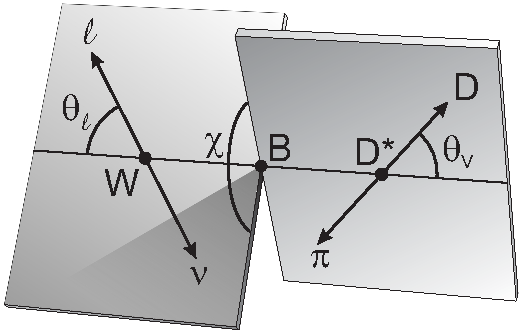
\includegraphics[width=0.65\textwidth]{./figs-theory/b_d_angular_vars.pdf}
    \caption{
        Angular variables of the $\Bzb \rightarrow D^{*+} \ellm\neulb$ decays.
        For $\Bm \rightarrow \Dz\ellm\neulb$ decays,
        only the $\theta_l$ variable exists.
    }
    \label{fig:b-d-decay-schematic}
\end{figure}

\paragraph{Leptonic current}
The leptonic currents are straightforward to evaluate,
as the weak interaction permits a perturbative calculation and the currents can
be sufficiently approximated by tree-level decays.
Evaluated in the $B$ rest frame, each lepton current of the polarization combintation
$(\lambda_W, \lambda_l)$ is a function of the lepton mass,
the invariant mass squared $q^2$ of the virtual $W$,
and $\theta_l$ as defined in \cref{fig:b-d-decay-schematic}.
The results are listed in eqs. (2.8) and (2.9) in
\cite{HAGIWARA1989569}, and are copied over with minor changes on notations:

\begin{align}
    & L^-_\pm(q^2, \theta_l) = -2 \sqrt{q^2} v d_\pm
    & L^-_0(q^2, \theta_l) &= -2 \sqrt{q^2} v d_0
    & L^-_s(q^2, \theta_l) &= 0
    \label{eqn:b-d-l-current-1} \\
    & L^+_\pm(q^2, \theta_l) = \mp \sqrt{2} m_l v d_0
    & L^+_0(q^2, \theta_l) &= \sqrt{2} m_l v(d_+ - d_-)
    & L^+_s(q^2, \theta_l) &= -2 m_l v
    \label{eqn:b-d-l-current-2}
\end{align}
where $v = \sqrt{1 - \frac{m^2_l}{q^2}}$,
$d_\pm = \frac{1 + \cos\theta_l}{\sqrt{2}}$, and $d_0 = \sin\theta_l$.

\paragraph{Hadronic current} The calculation of the hadronic currents, however,
involves non-perturbative quantum chromodynamics (QCD) effects as both the
initial and final states are mesons which are quark-anti-quark pairs bounded by
the strong interactions of QCD.
Hence, these currents are not computable in an analytical way and each of them
is re-expressed in terms of form factors (FFs),
which are a function of \qSq, instead.
These FFs are parameterized and estimated with relatively large theoretical
uncertainties with four types of methods:
use of functional properties of the matrix elements\footnote{
    Such as analyticity, unitarity, and dispersion relations.
},
heavy quark effective theory (HQET),
various quark models\footnote{
    For example QCD sum rule (QCDSR) and light cone sum rule (LCSR).
},
and lattice QCD
\cite{Bernlochner_2022}.
As mentioned in the introduction,
for \RDX ratio measurements,
the hadronic uncertainties are mostly factored out and the main importance
of the FFs lies in the precision of the lepton universality ratio predictions.
% NOTE: Check the slides for CLN vs. BGL
%   https://indico.cern.ch/event/656737/contributions/2676125/attachments/1525023/2384258/Siegen.pdf
The estimations of FFs
and the differential decay rate (which will be provided shortly after)
are often performed at a particular $q^2$ value, such as when the $D$ meson is
produced at rest in the $B$ rest frame\footnote{
    Referred to as ``zero recoil'' due to the fact that the $D$ meson is
    \emph{not recoiling} in the $B$ rest frame.
},
and are extrapolated to the full $q^2$ range by performing fits to experimental
inputs.

While not analytically calculable,
the hadronic currents are constrained by the conservation of angular momentum,
which implies that the $D$ and the virtual $W$ should have the same helicity.
For a $D^0$ meson, whose only possible helicity state is 0,
the only non-zero hadronic amplitudes are $H^0_0, H^0_s$.
For $D^*$ meson,
the amplitudes $H^+_+$ and $H^-_-$ are allowed in addition.

\paragraph{Differential decay rate}
The differential decay rate is found by first inserting
\cref{eqn:b-d-l-current-1,eqn:b-d-l-current-2}
into \cref{eqn:b-d-master-formula} then integrating over the phase space and
summing over the lepton helicities:

\begin{align}
    \frac{d\Gamma}{d q^2 d\cos\theta_l} =&
    \frac{G^2_F |V_{cb}|^2 | \vec{p}^*_D|^2 q^2}{256 \pi^3 m^2_B}
    \left(1 - \frac{m^2_l}{q^2}\right)^2 \times
    \nonumber \\
    &\bigg[
        (1 - \cos\theta_l)^2 |H_+|^2 + (1 + \cos\theta_l)^2 |H_-|^2 +
        2 \sin^2\theta_l |H_0|^2 +
    \nonumber \\
    & \frac{m^2_l}{q^2} \left(
        (\sin^2\theta_l(|H_+|^2 + |H_-|^2) + 2|H_s + H_0 \cos\theta_l|^2)
    \right)
    \bigg]
\end{align}
where the \qSq dependence and the helicities of the $D$ meson in the hadronic
currents $H_{\{\pm,0,s\}}$ are omitted.

In the next sections the form factor parameterizations relevant to this analysis
for \Dz, \Dstar, and \Dstst mesons are discussed.


\subsection{Form factors in $B \rightarrow \Dz\ellm\neulb$ decays}
\label{ref:theory:ff-d0-dst}

As discussed before,
a form factor parameterization of the hadronic currents is needed in order to
evaluate the differential decay rate.
In this analysis both \Dz and \Dstar MCs are generated with the CLN
parameterization and later reweighted offline to BGL.
More details will be given for \Dz parameterizations.
For \Dstar only the parameterization schemes and parameter values will be given.

\paragraph{CLN}
For $B \rightarrow \Dz$ decays the axial vector part of the hadronic current is
vanishing due to conservation of angular momentum and parity
\cite{Bernlochner_2022}.
Each hadronic current is therefore characterized by \emph{two} form factors:
\begin{align}
    \bra{D} \bar{c} \gamma^\mu(1 - \gamma^5) b \ket{B} &=
    \bra{D} \bar{c} \gamma^\mu b \ket{B}
    \nonumber \\
    &=
    \sqrt{m_B m_D} \left[
        h_+(w)(v_B + v_D)^\mu + h_-(w)(v_B - v_D)^\mu
    \right]
\end{align}
where $v_i = \frac{p_i}{m_i}$,
$w(\qSq) \equiv v_B \cdot v_D = \frac{m^2_B + m^2_D - \qSq}{2 m_B m_D}$.
%%%%
In CLN parameterization \cite{Caprini_1998},
the FFs $h_+, h_-$ are re-expressed as $V_1(w), S_1(w)$:
\begin{align}
    V_1(w) &= h_+(w) - \frac{m_B - m_D}{m_B + m_D} h_-(w) \\
    S_1(w) &= h_+(w) - \frac{m_B + m_D}{m_B - m_D} \cdot \frac{w-1}{w+1} h_-(w)
\end{align}
and an expression for $V_1(w)$ is obtained by first analytically continue $w$
outside the physical region in the complex plane, then a conformal mapping
\begin{equation}
    w \rightarrow z: z =
    \frac{\sqrt{w+1} - \sqrt{2}a}{\sqrt{w+1} + \sqrt{2}a}
\end{equation}
is performed such that the physical region is mapped inside the unit circle of
the complex $z$-plane.
With dispersion techniques based on first principles and additional
consideration from heavy quark symmetries to further reduce degrees of freedoms,
$V_1(z)$ is expressed in powers of $z$, known as ``$z$-expansion'', as:
\begin{equation}
    V_1(z) = V_1(1) \cdot \left[
        1 - 8 \rho^2_D z + (51 \rho^2_D - 10) z - (252 \rho^2_D - 84) z^3
    \right]
\end{equation}
where $V_1(1), \rho^2_D$ are FF parameters.



\paragraph{BGL}


\subsection{Form factors in $B \rightarrow D^{**}\ellm\neulb$ decays}
\label{ref:theory:ff-dstst}

\paragraph{ISGW2}

\paragraph{BLR}
